\section{Design}
\label{sec:design}

\system uses a capacity-adaptive piecewise architecture to reconcile dynamic
expert placement with graph replay. It routes once and then selects between two
expert-execution paths. When the routed set fits the persistent bank, \system
replays captured expert computation against fixed storage bindings. When a
prefill working set exceeds that capacity, it executes exact eager waves from
fixed transient banks and reassembles their outputs before native composition.
Both paths preserve the same routing semantics and versioned storage-lifecycle
rules. The eager overflow path is an explicit execution mode, not a fallback
from failed graph replay. The design must therefore preserve stable replay
bindings, execute routed expert sets that exceed the available execution-bank
capacity, and safely coordinate asynchronous storage reuse.

\subsection{Execution Model and Invariants}
\label{sec:design-model}

Consider one managed MoE layer. Its native router produces a set of routed
token--expert pairs
$P=\{(i,e,j,w)\}$, where $i$ is a token, $e$ is a layer-local logical expert,
$j$ is its top-$k$ position, and $w$ is its routing weight. Let $E(P)$ denote
the distinct experts in $P$. An execution bank has capacity $C$ and a fixed
set of device buffers $\mathcal{S}$ for expert-weight groups. Its bank-local
addressing contract maps active logical experts to local slots. Let
$\beta_r(e)=s$ denote the active bank-local binding consumed for expert $e$ in
wave $r$. The persistent replay path realizes $\beta_r$ through a fixed
indirection buffer $\mathcal{M}$; an overflow wave encodes bank-local slot IDs
in its wave plan. In the evaluated layouts, the weight groups are $W_{13}$ and
$W_2$. The addresses, shapes, and types of the persistent buffers form the
storage binding visible to captured expert computation.

A managed invocation follows the same logical path regardless of whether
$E(P)$ fits in one bank; capacity determines the number and execution mode of
its waves. First, a captured routing piece produces $P$ once. The runtime
inspects the complete $E(P)$, determines whether it fits, and constructs a
capacity-bounded plan. A fitting invocation uses the persistent bank and its
prebound captured expert piece. An overflowing prefill invocation instead
materializes each $E_r$ as a complete wave in one fixed transient bank and
executes the wave through the eager expert path. Staging and expert execution
repeat until every routed pair has executed; their outputs are then restored
to the original pair positions and passed to the native composition path.
With multiple transient banks, staging wave $r+1$ may overlap computation of
wave $r$.

Figure~\ref{fig:architecture} separates these two expert paths. An expert
execution instance is associated with one pre-established bank binding; the
runtime never retargets one captured graph to a different allocation. The
persistent expert piece therefore continues to reference its capture-time
binding, while overflow execution selects among fixed transient banks in the
eager wave path. In both cases the seam may change slot contents and the active
binding $\beta_r$, but it does not reallocate the selected bank.

\begin{figure*}[!t]
  \centering
  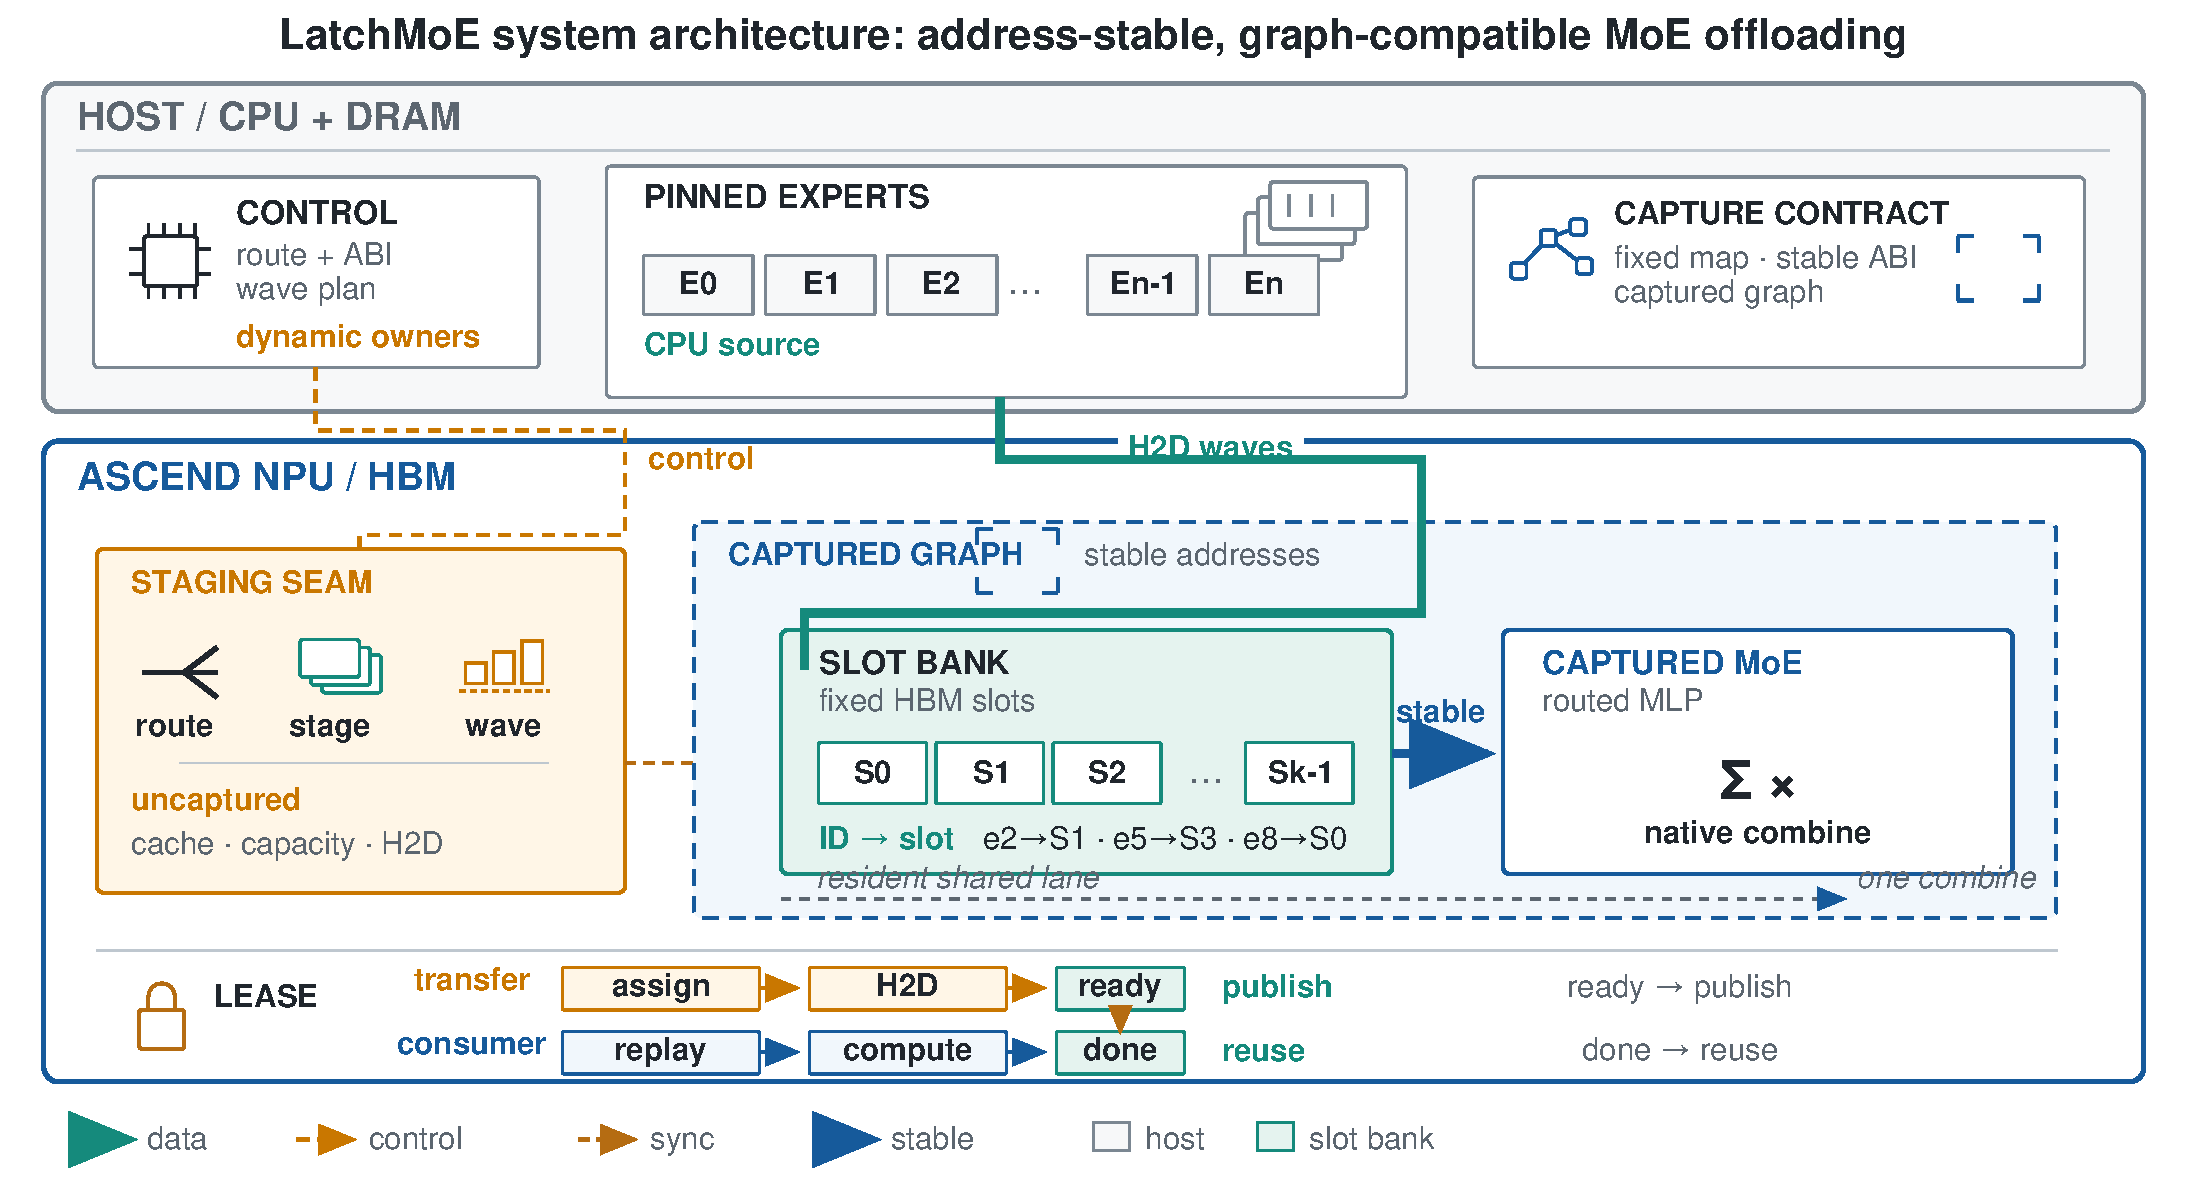
\includegraphics[width=\textwidth]{figures/latchmoe_architecture.pdf}
  \Description{LatchMoE routes once and plans the complete routed expert set.
  A fitting invocation stages into a persistent bank consumed by its captured
  expert piece. An overflowing invocation executes complete waves from fixed
  transient banks, then restores all wave outputs before native composition.}
  \caption{\system's route--plan--execute model. The persistent replay path is
  bound to one capture-time bank allocation. Overflow prefill uses complete
  waves in fixed transient banks rather than rebinding that captured piece.
  Both paths preserve the original routed pairs for one native composition.}
  \label{fig:architecture}
\end{figure*}

Correct execution rests on four invariants.

\begin{enumerate}[leftmargin=*, nosep]
\item \textbf{Stable replay bindings.} The persistent bank's weight buffers
  $\mathcal{S}$ and indirection buffer $\mathcal{M}$ retain the same
  allocations across capture and replay. Once allocated, transient banks are
  reused in place, but are not rebound into the captured expert path.
\item \textbf{Publish after readiness.} An active binding
  $\beta_r(e)=s$ becomes consumable only after the weights of expert $e$ are
  ready in slot $s$ for the current ownership version.
\item \textbf{Reuse after completion.} A slot cannot start its next ownership version until
  computation using its current version has completed.
\item \textbf{Exact routed semantics.} Every pair in $P$ executes exactly once
  with its original expert ID, top-$k$ position, and routing weight, even when
  $P$ is divided across waves.
\end{enumerate}

Together, the first invariant makes persistent placement changes compatible
with replay; the next two make asynchronous storage reuse safe on both paths;
the last preserves native MoE computation under capacity pressure.

\subsection{Stable Replay Bindings and Bounded Storage}
\label{sec:design-interface}

\paragraph{Expose routing without changing it.}
Staging cannot start until the active logical experts are known, but a
monolithic fused MoE operation hides selection inside the captured operation.
\system therefore relocates native selection into the first captured piece
rather than predicting or reimplementing it. This piece invokes the model's
native router with its configured parameters and emits the selected IDs and
weights. The seam may inspect IDs to plan waves and residency, but it cannot
add, drop, or rewrite routed entries. Both tensors continue unchanged to expert
execution, so routing is evaluated once and retains the model's native
decision.

\paragraph{Storage roles.}
Routed weights remain available in a host expert store. Each managed layer has
a layer-private persistent bank that preserves expert residency across
invocations, especially during decode. Overflow waves use transient banks as
bounded scratch storage, so staging a large prefill working set need not evict
the persistent working set. Compatible layers may share the transient-bank
pool because their executions are serial, whereas persistent banks remain
layer-private to retain temporal reuse.

The banks do not form one global slot namespace. The persistent bank and each
transient bank expose separate fixed weight buffers and bank-local addressing;
a plan selects one such pre-established binding and uses slot IDs local to that
bank. The captured expert piece is bound only to the persistent bank selected
at capture; choosing transient Bank A or B selects the eager wave path against
that fixed bank rather than rebinding the captured piece. Reassignment changes
buffer contents, ownership metadata, and active indirection values, but not
bank allocations. Logical IDs are also layer-local: equal numeric IDs in
different layers do not imply shared weights or residency.

The shared expert, when present, follows a separate lane. Because it is used by
every applicable token, \system leaves it device-resident and executes it once
per invocation. It neither consumes routed-slot capacity nor participates in
victim selection or wave partitioning.

\paragraph{Stage, then publish.}
After the router piece completes, the runtime first inspects the complete
routed set $E(P)$ to determine persistent hits, detect overflow, partition
waves, and select their execution banks. Materialization is then local to the
current route or wave rather than to all of $E(P)$. On the fitting replay path,
a ready hit retains its persistent slot; for a miss, the runtime selects a
reassignable persistent slot, removes its previous owner from the authoritative
residency metadata, advances its ownership version, and starts the H2D weight
transfer.

On the overflow path, every expert in $E_r$ is assigned a bank-local transient
slot so that one bank supplies the complete wave. A persistent hit is copied
device-to-device into that slot, whereas a miss is copied from the host store.
The transient slot's ownership version advances in either case. Only after all
required transfer dependencies are satisfied and each slot still matches its
issued owner and version does the runtime mark the binding ready and publish
$\beta_r$, making its bank-local slot IDs consumable by expert execution.

On the replay path, the device indirection buffer is a consumption interface,
not the authoritative residency directory. Its entries outside the active
route are unspecified and may retain values from an earlier invocation because
captured computation cannot reach them. On the overflow path, $\beta_r$ is
instead encoded by the current wave's bank-local slot IDs. Thus, for either
interface, only bindings reachable by the current expert operation must be
valid; inactive entries are semantically irrelevant. Before execution, every
active $\beta_r(e)=s$ must name a ready slot with a matching owner and version.
Publishing an active binding before readiness could expose partially
transferred weights; accepting completion for another ownership interval could
publish the wrong expert. Hits and misses nevertheless leave the seam through
the same bank-local storage contract.

\subsection{Exact Execution beyond Slot Capacity}
\label{sec:design-waves}

Stable bindings alone do not handle an invocation whose routed working set
exceeds $C$. Let $E=E(P)$. When $|E|>C$, \system partitions the expert set into
$E_1,\ldots,E_m$ and derives each wave's routed pairs:
\begin{equation}
\begin{aligned}
  &\bigcup_{r=1}^{m} E_r=E, \qquad
  E_r\cap E_q=\varnothing\ (r\ne q), \qquad |E_r|\le C,\\
  &P_r=\{(i,e,j,w)\in P\mid e\in E_r\}.
\end{aligned}
\end{equation}
Thus, all pairs for one expert remain in the same wave, and every pair in $P$
belongs to exactly one $P_r$. The partitioner may change expert execution
order, but not pair membership, top-$k$ positions, or routing weights. This is
tiling the expert dimension rather than approximating routing semantics.

Once overflow selects multi-wave execution, each $E_r$ is materialized in full
in one transient bank. Ready experts are copied from the persistent bank and
misses from the host store; expert computation never mixes weights from both
banks within one wave. This deliberate D2D copy preserves one coherent
bank-local binding and leaves persistent cache residency undisturbed. Since
each wave contains at most $C$ experts, bounded scratch storage can be reused
to cover the larger routed set.

Each wave computes only its assigned pairs and records their original pair
positions. After all waves finish, \system reassembles the routed contributions
at those positions and invokes the model's native composition path with the
original weights and output shape. The shared lane, if present, is computed
once and combined only after the routed contribution is complete. Consequently,
wave boundaries do not duplicate shared work or change model-specific routed
scaling, reduction, or postprocessing. Coverage validation treats a missing or
duplicate pair as an execution error.

For example, with $C=2$, the routed set $\{e_2,e_5,e_8\}$ requires at least
two waves. Every expert's routed pairs remain intact within one wave and are
restored to their original positions before native composition.

\subsection{Safe Transfer--Compute Overlap}
\label{sec:design-lifecycle}

Serially staging every wave would expose transfer latency. \system overlaps
the transfer of wave $k+1$ into Bank B with computation of wave $k$ from Bank
A, as shown in Figure~\ref{fig:lifecycle}(a). Bank A can then receive wave
$k+2$, but only after wave $k$ has stopped reading it. The same rule applies to
individual persistent slots and to whole transient banks.

\begin{figure*}[!t]
  \centering
  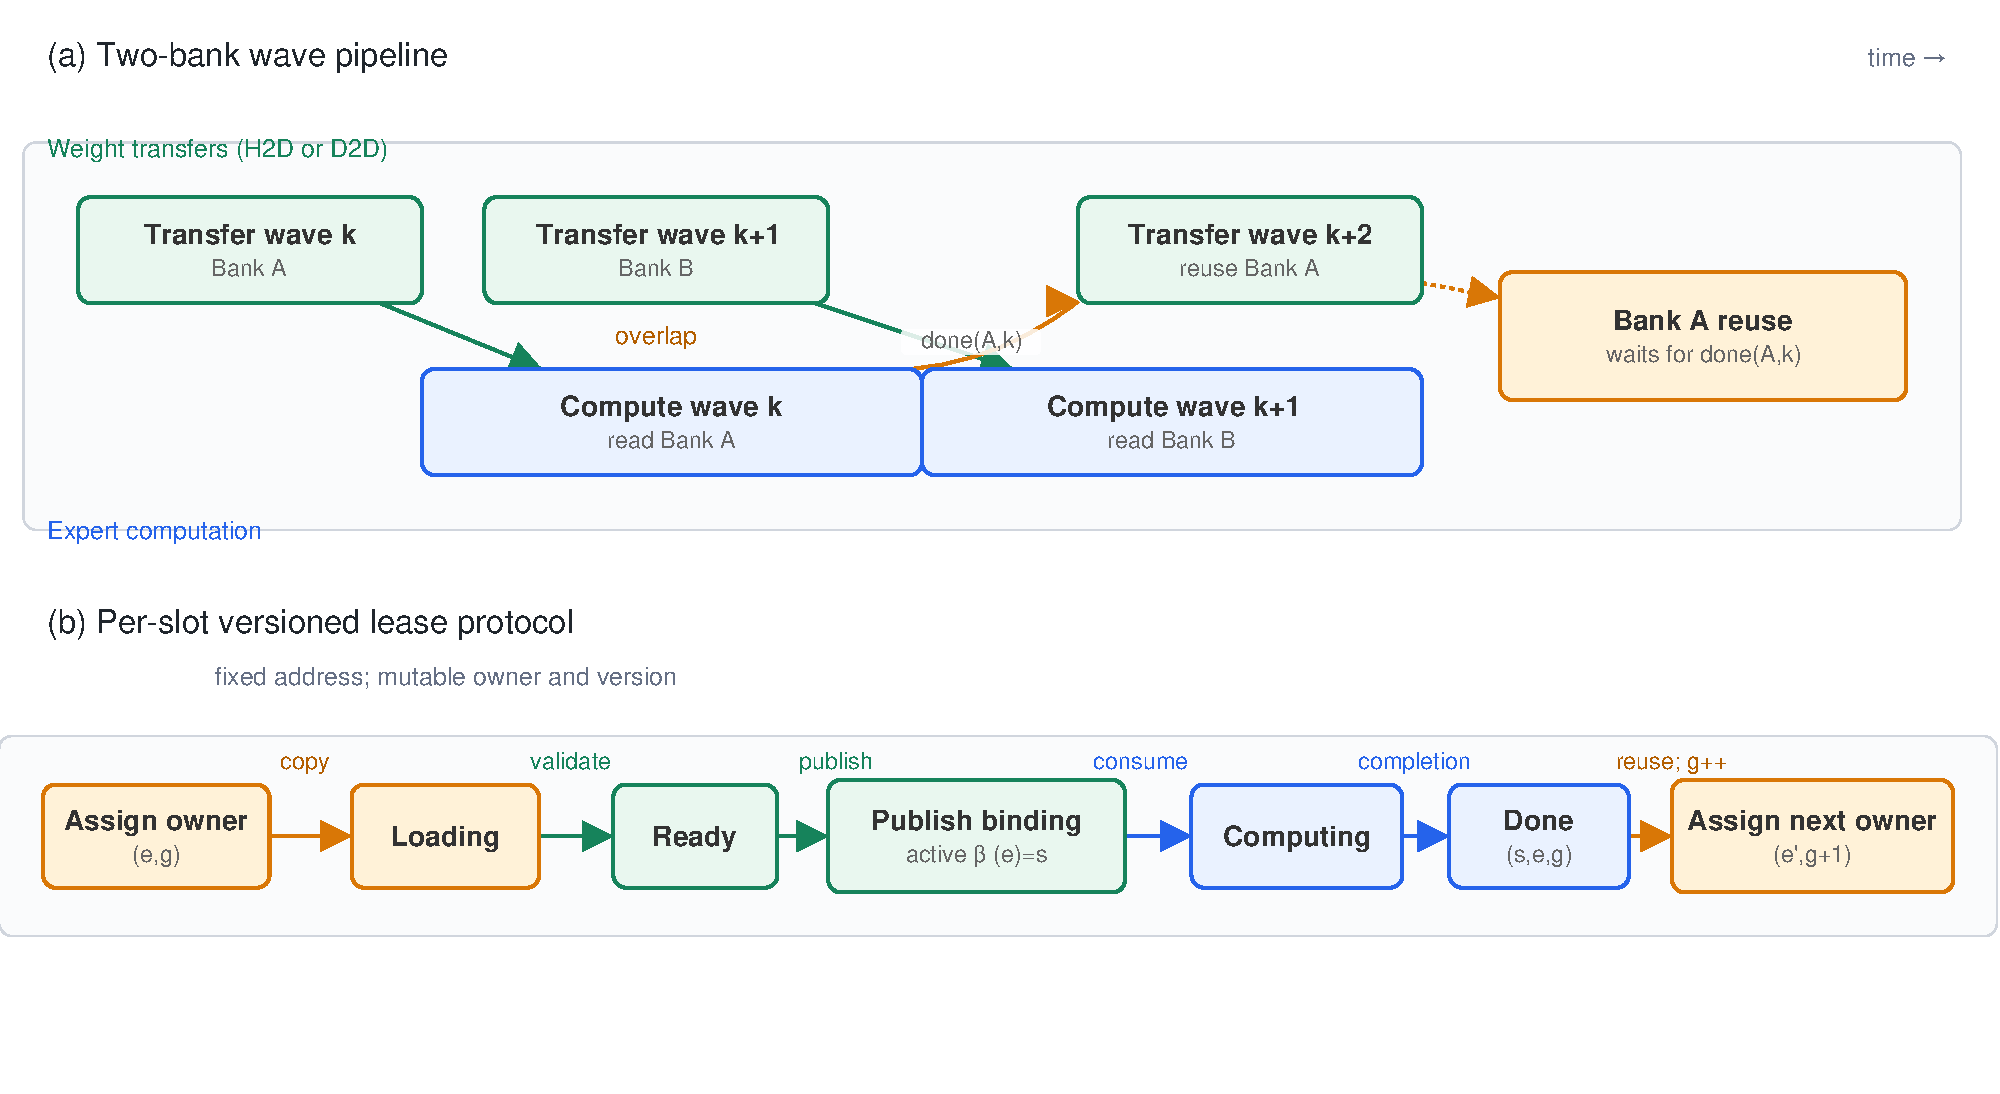
\includegraphics[width=\textwidth]{figures/latchmoe_lifecycle.pdf}
  \Description{The upper panel shows transfer of wave k plus one into Bank B
  overlapping computation of wave k from Bank A. Bank A is reused for wave k
  plus two only after wave k completes. The lower panel orders assignment,
  loading, readiness, publication, computation, completion, and reassignment.}
  \caption{Versioned leases order asynchronous staging and bounded reuse.
  (a) Two banks pipeline consecutive waves; a bank's next transfer waits for
  its previous compute completion. (b) The active binding is published only
  after transfer readiness and consumed only after publication; reassignment
  waits until no computation holds the current lease.}
  \label{fig:lifecycle}
\end{figure*}

Each slot carries a fixed device-buffer address and mutable
$(\mathit{owner},\mathit{version},\mathit{state})$ metadata. Its state is one
of \emph{empty}, \emph{loading}, \emph{ready}, or \emph{computing}. Assignment
of expert $e$ to slot $s$ advances the version to $g$, enters loading, and
returns a readiness event for the lease
$\lambda=(s,e,g)$. A loading slot is never selected for another assignment.
When the transfer-completion dependency is satisfied, the runtime validates
$\lambda$, enters ready, and may publish the active binding. Expert
computation starts only after that publication, acquires the ready lease, and
moves it to computing. Here,
\emph{computing} denotes one outstanding expert-operation lease for the current
slot version; that operation may contain routed pairs from several batched
requests. A subsequent operation cannot acquire or reassign the slot until the
completion event returns it to ready. The slot does not become empty merely
because one use completes, since retaining its owner enables a future cache
hit.

The protocol imposes the following happens-before relations:
\begin{equation}
\begin{aligned}
  \operatorname{ready}(s,e,g) &\prec
  \operatorname{publish}(\beta_r(e)=s)
  \prec \operatorname{compute}(s,e,g), \\
  \operatorname{done}(s,e,g) &\prec
  \operatorname{assign}(s,e',g+1).
\end{aligned}
\end{equation}
The first chain prevents incomplete or unpublished weights from being
consumed. The second prevents a new transfer from overwriting weights still
consumed by a kernel.
Normal scheduling therefore reassigns neither loading nor computing storage.
Owner/version checks additionally reject a delayed event from an earlier
ownership interval instead of allowing it to authorize publication or reuse.

At bank granularity, the same lease rule gives a simple pipeline. Transfer
into Bank B may proceed while Bank A is computing because the banks are
disjoint. Reusing Bank A for wave $k+2$ waits specifically for the completion
event of wave $k$; it need not serialize on unrelated work in Bank B. This
coordination exposes exactly the dependencies needed for safety while leaving
independent transfer and compute eligible to overlap.

\subsection{Design Boundary}
\label{sec:design-boundary}

\system separates execution correctness from placement quality. A placement
policy may choose residency, wave membership, and execution order only over the
complete routed expert set; it cannot add or remove routed experts or alter
capacity constraints, publication, or lease rules. The split interface is
enabled only for supported router, shared-expert, and output contracts, while
unsupported contracts are rejected rather than approximated. Concrete
combinations of model and runtime still require semantic and replay
qualification, which Section~\ref{sec:evaluation} reports.
